Local development of the project was designed to be easy to set up and reproducible in any development machine. For this purpose development virtual machine(referred as dev-VM) was created using the infrastructure-as-a-code principle. Tools which are used for reproducible creation of machine are:
\begin{itemize}
    \item Oracle Virtualbox\cite{virtual_box} - hypervisor which is hosting VM, it was chosen because it supports deployment in the 3 most popular operating systems: Microsoft windows, mac os, and Linux.
    \item HashiCorp Vagrant\cite{vagrant} - a tool that helps to build a development environment as a code. It allows specifying all details of provisioned VM, as well as configuring networking and hardware specifications. All files used for development can be found in dev-VM repository\cite{dev_vm}.
\end{itemize}

The base of the development virtual machine is an Ubuntu Linux server, so it is not shipped with the graphical user interface. It was chosen to resemble the production environment, lower the VM blueprint and increase the speed and performance of the setup. To interact with the machine Secure Shell Protocol (SSH) is used, it can be seen in picture \ref{fig:local_development}.

\begin{figure}[H]
    \centering
    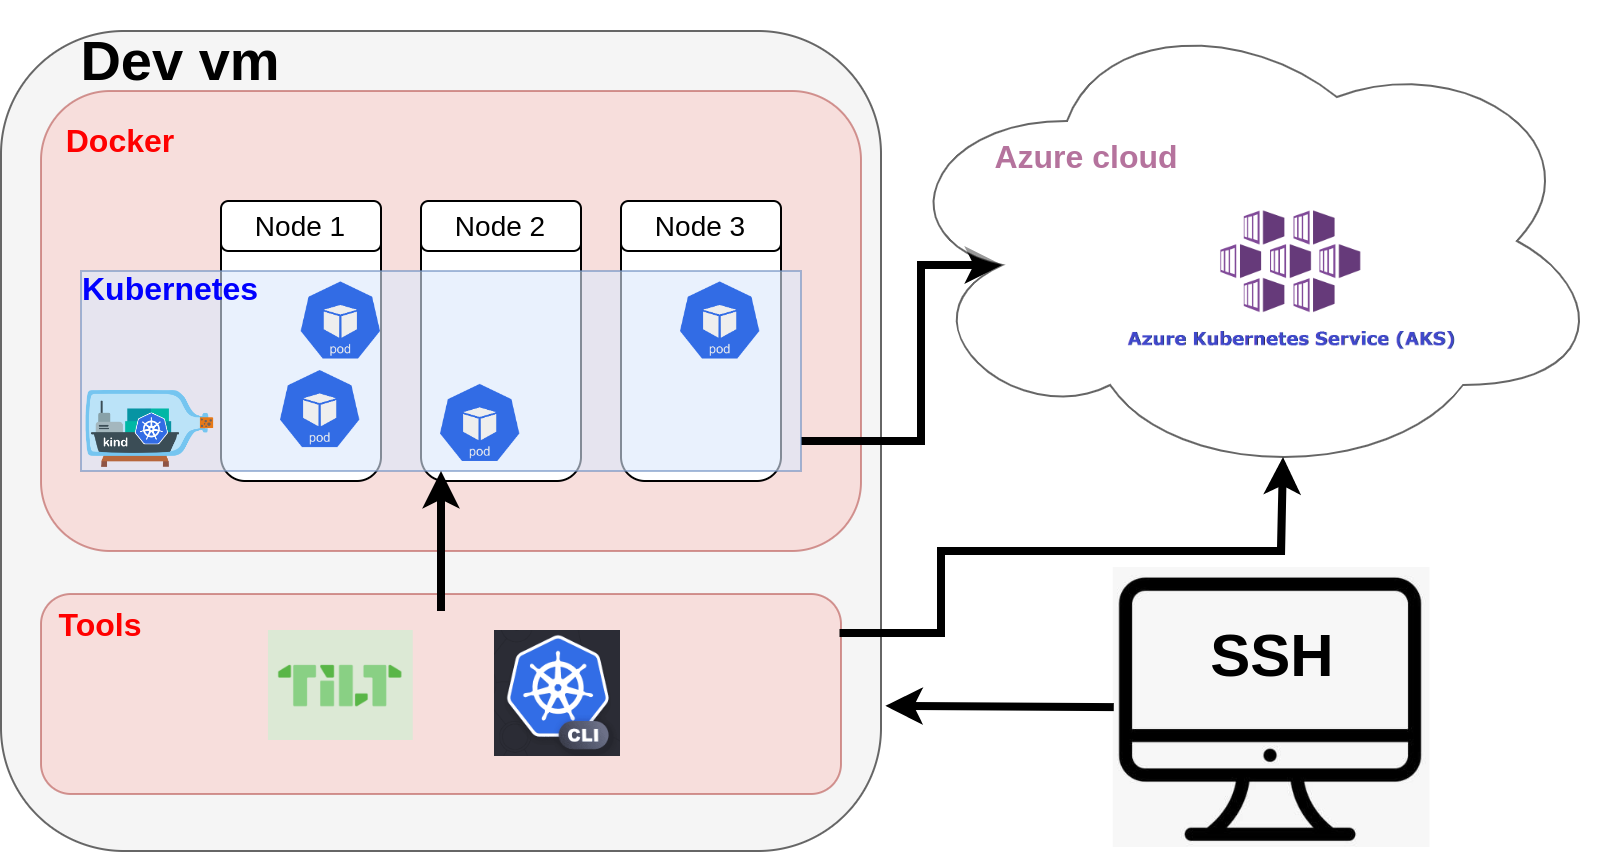
\includegraphics[width=0.8\textwidth]{pictures/development_setup.png}
    \caption{ Local development }
    \label{fig:local_development}
\end{figure}

By default Kubernetes(k8s) cluster is deployed in dev-VM using a tool called 'kind'. It allows the creation of Kubernetes nodes as containers and forms a Kubernetes (k8s) cluster. It can be then accessed with Kubernetes client command line tool called 'kubectl'. To speed up the development process and allow continuous testing of both software and deployment, software called tilt is used. This software interacts with the k8s cluster by building container images and deploying resources as soon as there is any change in the code. It also includes a dashboard \ref{fig:tilt} which visualizes resources deployed in a cluster as well as aggregates the logs and shows them in an approachable matter.


\begin{figure}[H]
    \centering
    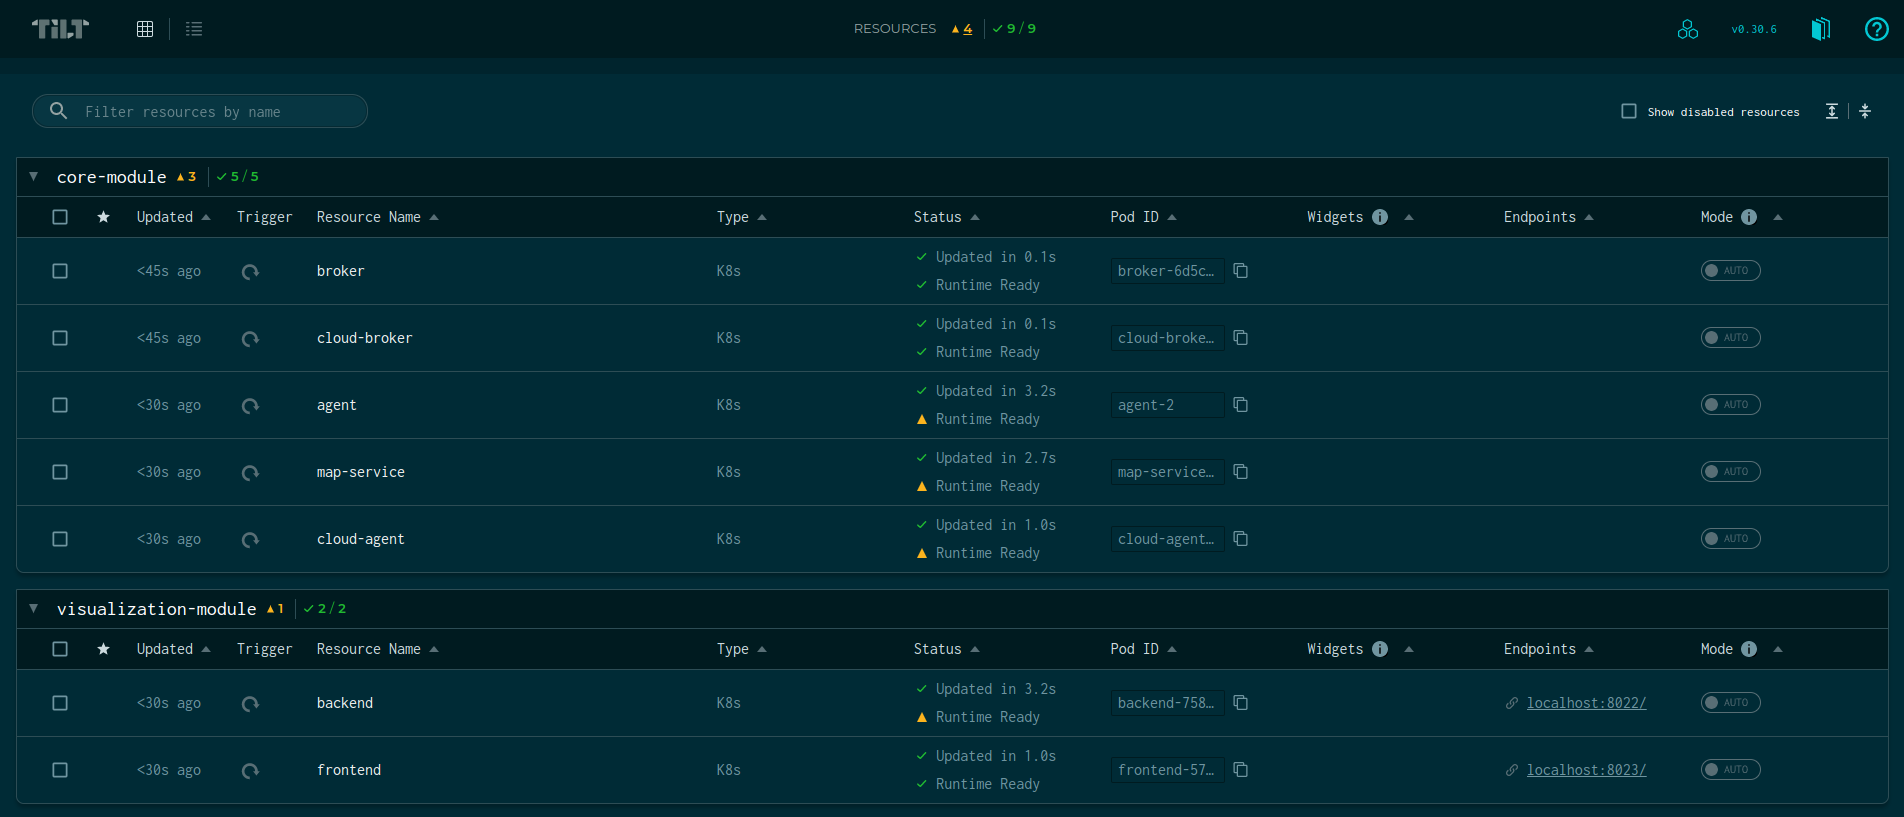
\includegraphics[width=\textwidth]{pictures/tilt.png}
    \caption{ Tilt dashboard}
    \label{fig:tilt}
\end{figure}

Integration with an azure cloud is made with azure command lines tools along with PAT token. After the initial creation of the Kubernetes cluster in the cloud, interactions are limited to only the Kubernetes cluster and therefore only kubeconfig(Kubernetes configuration) file is needed.

In order to improve the ease of interaction with the various resources used in the project, a set of "make rules" were developed. These rules abstract the workflow by consolidating multiple commands into logical components referred to as "rules" or "targets." The entirety of the rules are documented in the appendix \ref{sec:app_05}.
